 \begin{motivating}
    What is the definition of the integral in single variable calculus? 
    \end{motivating}
    

\section{Defining the integral}

\begin{motivating}
    What is the definition of the integral in single variable calculus? 
\end{motivating}

PICTURE

    \begin{enumerate}
        \item Can we define the integral such that we can deal with both  $\int_\infty^\infty f(x) \ dx$ and $\int_a^b f(x) \ dx$?
        \item Can we define the integral in a way that easily generalizes to multivariable functions $f: \R^n \to \R$?
        \item What kinds of functions can we integrate? 
    \end{enumerate}

In these lecture notes, we'll be dealing with proper/definite integrals.  That is, we will want our integrals to have finite values.\footnote{It takes some care to define non-proper integrals in multivariable calculus!}

That is, we'll be working with functions that are \textbf{bounded} with \textbf{bounded support}.

\begin{definition}
A subset $D \subset \R^n$ is \textbf{bounded} if there exists some $r > 0$ such that $D \subset B_r(\bm{0})$.
\end{definition}

\fixthis{recall}
    
    
    \begin{definition}
    A function $f: A \subset \R^n \to \R$ is \textbf{bounded}\define{bounded function} if its image $$\{f(\bm{x}) \ | \ \bm{x} \in A \}$$ is a bounded subset of $\R$.
    \end{definition}

\fixthis{recall}

\begin{definition}
A point $\bm{x} \in \R^n$ is a \textbf{boundary point} of $D \subset \R^n$ if: for all $\varepsilon > 0$,

\begin{enumerate}
    \item $B_\varepsilon(\bm{x}) \cap D$ is non-empty, \textbf{and}
    \item $B_\varepsilon(\bm{x}) \cap D^{c}$ is non-empty.
\end{enumerate}
\end{definition}
    
    \begin{definition}
    The \textbf{closure} of a set $D \subset \R^n$ is the union of $D$ and the boundary of $D$.  That is, the closure is the set $$\overline{D} = \{\bm{x} \in \R^n \ | \ B_r(\bm{x}) \cap D \neq \varnothing \textnormal{ for all } r\in\R \}$$  
    \end{definition}

\begin{proposition}
    A set $D$ is closed (\fixthis{recall}) if and only if $$D = \overline{D}$$
\end{proposition}

\begin{definition}
    The \textbf{support}\define{support of a function} of a function $f : A \subset \R^n \to \R$ is the \textbf{closure} of the set $$\{\bm{x} \in A \ | \ f(\bm{x}) \neq 0\}$$
\end{definition}

\begin{definition}
    A function has \textbf{bounded support}\define{bounded support} if its support is bounded.  

    Equivalently, there exists $R>0$ such that $f(\bm{x}) = 0$ for all $||\bm{x}|| > R$.
    \end{definition}

We can now define the notion of multivariable integral for bounded functions with bounded support.  


\subsection{Integration over $\R^n$}

The main idea of integrating a function $f: \R^n \to \R$ is not so difficult: 

\begin{enumerate}
    \item We chop up our region into pieces.
    \item We sample $f$ on each of the pieces, and sum over the pieces.
    \item We take the limit of the sum as the size of the pieces shrinks.
\end{enumerate}

However, \textbf{we will need to be careful}, as we will encounter some technical difficulties in making these ideas rigorous.


We will begin with chopping up the domain of $f$ (e.g. $\R^n$) into pieces.  In technical terms, we will construct a \textbf{partition} of $\R^n$.

\begin{definition}
    A \textbf{partition} of a set $X$ is a collection of non-empty subsets $X_\alpha \subset X$ such that every elemnent of $x \in X$ is in \textbf{exactly one} $X_\alpha$.
\end{definition}

\begin{definition}
    Given a vector $\bm{k} = \langle k_1, \cdots, k_n\rangle \in \Z^n \subset \R^n$ (that is, $k_i \in \Z$ for all $i$), we can define the \textbf{dyadic cube} $C_{\bm{k},N}$ in $\R^n$ as
    $$C_{\bm{k},N} := \left\{ \bm{x} = \langle x_1, \cdots, x_n\rangle \in \R^n \ | \ \frac{k_i}{2^N} \leq x_i < \frac{k_i+1}{2^N}\right\}$$
    
    \end{definition}

\begin{example}

        What is the dyadic cube $C_{1,1}$ in $\R^1$?
        
        What is the dyadic cube $C_{1,2}$ in $\R^1$?
    

\fixthis{picture}
    
        What is the dyadic cube $C_{\langle1,1\rangle,1}$ in $\R^2$?

\end{example}





\begin{proposition}
    The volume of a dyadic cube $C_{\bm{k},N}$ in $\R^n$ is $\frac{1}{2^{Nn}}$.
    \end{proposition}

\begin{proposition}
    For a fixed $N$, the collection of all dyadic cubes $$D_N(\bm{\R^n}) := \left\{C_{\bm{k},N} \ | \ \textnormal{for all} \ \bm{k} \in \Z^n \right\}$$ partitions $\R^n$. We call $D_N(\bm{\R^n})$ the $N$\textbf{-th dyadic partition of} $\R^n$.
    \end{proposition}





The dyadic partition is a convenient choice of \textbf{partition} of $\R^n$. We have chosen this particular partition as it is systematic and easy to define.

There are many other ways to partition $\R^n$, and they each lead to an equivalent definition of the multivariable integral.  For example, it turns out that the partitions do not need to be uniform (e.g. we could take rectangles with differing widths).  Moreover, we could take partitions depending on the range of the function (this leads to the notion of the Lebesgue integral).

 


Given our dyadic cube partition, we now turn to sampling points from the partition:

\fixthis{lower left corner, midpoint, etc.}

\begin{definition}\label{def:riemannsum}
    Given a choice of $\bm{x_{k,N}} \in C_{\bm{k},N}$ for every cube, the $N$-th \textbf{Riemann sum}\define{Riemann sum} is defined as 
    $$R_N(f) := \sum_{C \in D_N(\R^n)} f(\bm{x_{k,N}}) \ \textnormal{vol(C)}$$
    \end{definition}

We have many choices for sampling points, and it is a priori unclear that these various sampling methods should produce the same value for our integral when we take the limit as $N$ goes to $\infty$.

Thus, we will use Darboux sums to define the multivariable integral - this will guarantee that if the limit as $N$ goes to $\infty$ exists, then any sampling method will produce the same value\footnote{See proposition \ref{prop:riemannisintegrable} and exercise \ref{problem:riemannintegrabletodarboux}}.

 \begin{definition}
    Let $X \subset \R$.  A number $M \in \R$ is an \textbf{upper bound of $X$}\define{upper bound} if for every $x \in X$, we have that $x \leq M$.  
 
    \end{definition}

\begin{definition}   
    Let $q$ be an upper bound of $X$. We say $q$ is the \textbf{supremum of $X$}\define{supremum} (or \textbf{least upper bound of $X$}\define{least upper bound}) if for all upper bounds $M$ of $X$, we have that $q \leq M$.
    
    We write $q := \sup(X)$.  If $X$ is not bounded above, we write $\sup(X) = \infty$.
    
    \end{definition}

\begin{definition}
    Let $X \subset \R$.  A number $m \in \R$ is an \textbf{lower bound of $X$}\define{lower bound} if for every $x \in X$, we have that $m \leq x$.  
 
    \end{definition}

\begin{definition}
    Let $p$ be a lower bound of $X$. We say $p$ is the \textbf{infimum of $X$}\define{infimum} (or \textbf{greatest lower bound of $X$}\define{greatest lower  bound} ) if for all lower bounds $m$ of $X$, we have that $m \leq p$.
    
    We write $p := \inf(X)$.  If $X$ is not bounded below, we write $\inf(X) = -\infty$.
    
    \end{definition}

    
    \begin{example}
        Consider the set $X = \{\frac{1}{n} \ | \ n \in \N \}$.  What is $\sup(X)$ and  $\inf(X)$?
    \end{example}

    We would often like to describe the largest and smallest element of a subset of $\R$.  However, if we consider sets like $X = \{1-\frac{1}{n} \ | \ n \in \N \}$ and $Y = \{\frac{1}{n} \ | \ n \in \N \}$, we see immediately that there is no largest elemnt in $X$, and that there is no smallest in $Y$.  Thus, we need to use the notions of the supremum and infimum, instead.


    

    \begin{theorem}[Completeness of $\R$]\label{thm:completness}
    Every nonempty subset $X \subset \R$ has a supremum and infimum. Moreover, $\sup(X)$ and $\inf(X)$ are unique.
    \end{theorem}



    \begin{definition}
    Let $f: \R^n \to \R$ be a function, and $D \subset \R^n$ an arbitrary subset. We will consider the following quantities:
    $$M_D(f) := \sup(\{f(\bm{x}) \ | \ \bm{x} \in D\}) \qquad m_D(f) := \inf(\{f(\bm{x}) \ | \ \bm{x} \in D\})$$
    
    \end{definition}

    \begin{example}
        Consider the subset $C_{1,2}$ in $\R^1$, and let $f(x) = \frac{1}{x}$.  
        
        Calculate $M_{C_{1,2}}(f)$ and $m_{C_{1,2}}(f)$.
    \end{example}


    
    \begin{definition}
    Let $f: \R^n \to \R$ be a bounded function with bounded support. The $N$\textbf{-th upper Darboux sum} and $N$\textbf{-th lower Darboux sum} $f$ are defined as 
    $$U_N(f) := \sum_{C \in D_N(\R^n)} M_C(f)\textnormal{vol(C)} \qquad L_N(f) := \sum_{C \in D_N(\R^n)} m_C(f)\textnormal{vol(C)}$$
    
    \end{definition}

    \begin{center}
        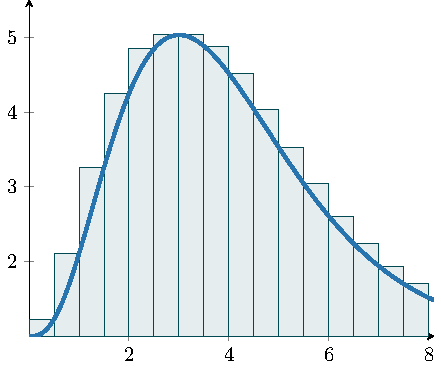
\includegraphics{chapters/4-IntegrationRn/figures/figures-upperdarboux.pdf}
        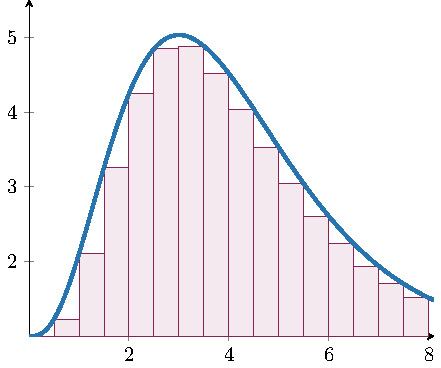
\includegraphics{chapters/4-IntegrationRn/figures/figures-lowerdarboux.pdf}
    \end{center}

    \begin{proposition}
    $$U_N(f) := \frac{1}{2^{Nn}} \sum_{C \in D_N(\R^n)} M_C(f)  \qquad L_N(f) := \frac{1}{2^{Nn}}\sum_{C \in D_N(\R^n)} m_C(f)$$
    \end{proposition}
    
    \begin{proposition}
    As $N$ increases, $U_N(f)$ decreases and $L_N(f)$ increases.
    \end{proposition}

    \begin{center}
        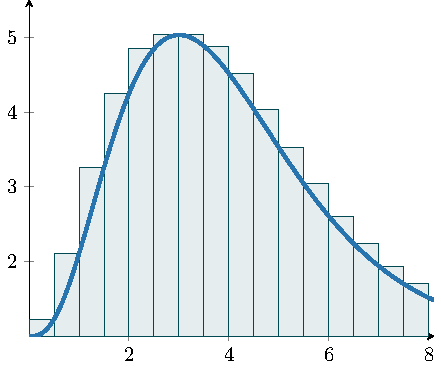
\includegraphics{chapters/4-IntegrationRn/figures/figures-upperdarboux.pdf}
        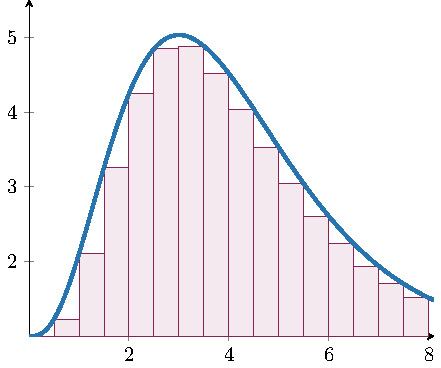
\includegraphics{chapters/4-IntegrationRn/figures/figures-lowerdarboux.pdf}
    \end{center}

    \begin{center}
        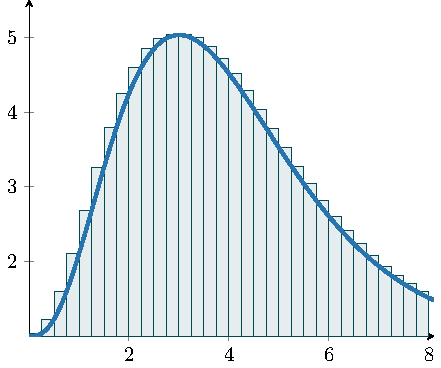
\includegraphics[scale=0.7]{chapters/4-IntegrationRn/figures/figures-upper2.pdf}
        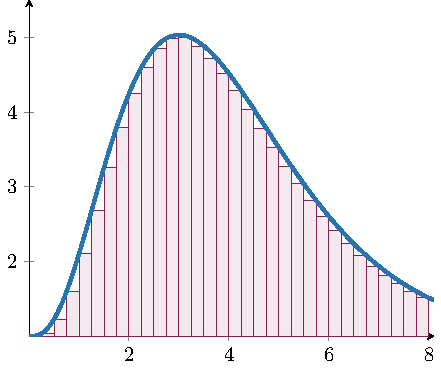
\includegraphics[scale=0.7]{chapters/4-IntegrationRn/figures/figures-lower2.pdf}
    \end{center}
    
    
    \begin{definition}
    Let $f: \R^n \to \R$ be a bounded function with bounded support.  The \textbf{upper Darboux integral} and \textbf{lower Darboux integral} of $f$ are defined as
    $$U(f) := \lim_{N \to \infty} U_N(f)   \qquad L(f) := \lim_{N \to \infty} L_N(f)$$
    \end{definition}

    \begin{remark}
        \fixthis{limits exist}
    \end{remark}

\begin{definition}\label{def:integrable}
    Let $f: \R^n \to \R$ be a bounded function with bounded support.
    We say that $f$ is \textbf{integrable}\define{integrable} if $U(f) = L(f)$.
    
    The \textbf{integral} of $f$ is $$\int_{\R^n} f(\bm{x}) \ dV := U(f) = L(f)$$

    By proposition \ref{epsilonenough}, this equivalent to asking that for any $\varepsilon > 0$,
    there exists $N$ such that $|U_N(f) - L_N(f)| < \varepsilon$
    \end{definition}

    

    
    \begin{corollary}
    If $f$ is integrable, we can use $U_N(f)$ or $L_N(f)$ to estimate $\int_{\R^n} f(\bm{x}) \ dV$. 
    \end{corollary}


\begin{motivating}
    How should we interpret our definition of the integral?
\end{motivating}

\begin{remark}
    If $f(\bm{x})$ is positive, then the integral is the $n$-dimensional volume under the graph of $f(\bm{x})$.  Otherwise, we can think of the integral as being the \textbf{signed} volume under the graph of $f(\bm{x})$.

    \begin{center}
        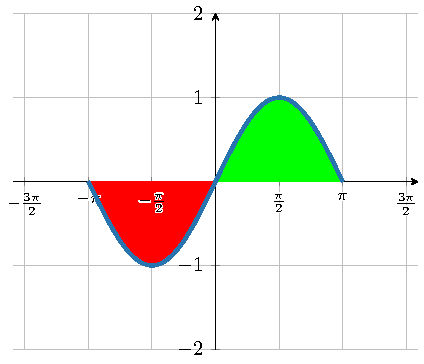
\includegraphics{chapters/4-IntegrationRn/figures/figures-signedvolume.pdf}
    \end{center}
\end{remark}

\begin{motivating}
    What functions are integrable?
\end{motivating}

    \begin{example}
    \begin{theorem}
     If $f : \R^n \to \R$ is a continuous function that is bounded with bounded support, then $f$ is integrable.   
    \end{theorem}
    \end{example}

    
However, there are some functions that are ``obviously" integrable, yet are not continuous:

\begin{example}
    Consider the unit square $A = [0,1] \times [0,1] \subset \R^2$.   We can define an indicator function to be the function $1_A  :\R^n \to \R$ is the function 
    $$1_A(\bm{x}) := \left\{
		\begin{array}{ll}
			1 & \text{ if } \bm{x} \in A \\
			0 & \text{ if } \bm{x} \notin A
		\end{array}
		\right.$$

  We expect the integral of $1_A(\bm{x})$ to give us the area of $A$.  However, this function is not continuous.
\end{example}
    
    In section \ref{sec:integrability}, we will discuss criteria for a function $f$ to be integrable.  For now, whenever we say integrable, you should think of continuous functions that are bounded with bounded support.



\begin{remark}
Note that if the integral $\int_{\R^n} f \ dV$ exists, then these two boundedness conditions($f$ is bounded and $f$ has bounded support) guarantee that the integral is finite.    
\end{remark}



\begin{remark}
    Using the Darboux formulation, it follows that if $f$ is integrable, then any choice of sampling  \fixthis{will result in the same value for the integral}
\end{remark}

\begin{proposition}\label{prop:riemannisintegrable}
    If $f: \R^n \to \R$ is integrable, then the integral is the limit of the Riemann sum.  

    Recall that given a choice of $\bm{x_{k,N}} \in C_{\bm{k},N}$ for every cube, the $N$-th \textbf{Riemann sum}\define{Riemann sum} is defined as 
    $$R_N(f) := \sum_{C \in D_N(\R^n)} f(\bm{x_{k,N}}) \ \textnormal{vol(C)}$$
    This yields the \textbf{Riemann integral}
    $$\lim_{N \to \infty} R_N(f) = \int_{\R^n} f(\bm{x}) \ dV$$
    \end{proposition}

    \begin{example}
        For example, we can choose the \textbf{midpoint rule} by choosing $$\bm{x_{k,N}} = \langle \frac{2k_1 + 1}{2^{N+1}}, \cdots, \frac{2k_n + 1}{2^{N+1}} \rangle $$

        \begin{center}
            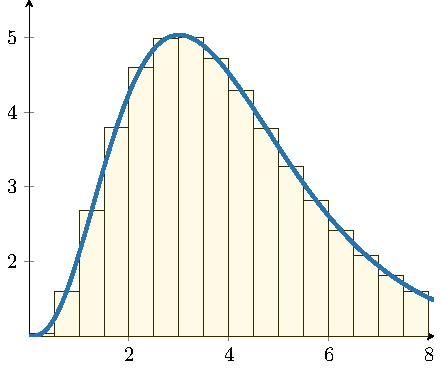
\includegraphics{chapters/4-IntegrationRn/figures/figures-riemannmidpoint.pdf}
        \end{center}
    \end{example}

    
    \begin{example}
     \textbf{Warning!} This only works if you know $f$ is integrable.  The Riemann sum may converge even if the function is not integrable.  Consider the function: $$f(x) := \left\{
		\begin{array}{ll}
			1 & \text{ if } x \in [0,1] \text{ and }  x \notin \Q \\
			0 & \text{ otherwise}
		\end{array}
		\right.$$   
    \end{example}


\subsection{Integration over subsets of $\R^n$}

Observe that we have defined the analogue of $\int_{-\infty}^\infty f(x) \ dx$ in single variable calculus.

    \begin{motivating}
        How can we define the analogue of $\int_a^b f(x) \ dx$?  
    \end{motivating}

    In other words, how do we integrate over sub-regions of $\R^n$?

    Suppose that $B \subset \R^n$ is a region in $\R^n$.  We have two potential ways to define the integral of $f$ over $B$ (denoted $\int_B f \ dV$).  We can either:

    \begin{enumerate}
        \item incorporate $B$ into the definition of the integral $\int_B f \ dV$.        
    In other words, given any subset $B$, we would need to partition $B$ into smaller subsets, and take a limit.
        \item or we can treat $B$ as part of the \textbf{input} of the integral.
        That is, we can use the partition of $\R^n$ that we constructed previously to yield a partition of $B$.
        
    \end{enumerate}

    We will take the second perspective, and define the integral of $f$ over $B$ in terms of some integral $\int_{\R^n} g \ dV$.  We can do so using \textbf{indicator functions}:

    \begin{definition}
    Let $B \subset \R^n$ be a subset.  The \textbf{indicator function} $1_B  :\R^n \to \R$ is the function 
    $$1_B(\bm{x}) := \left\{
		\begin{array}{ll}
			1 & \text{ if } \bm{x} \in B \\
			0 & \text{ if } \bm{x} \notin B
		\end{array}
		\right.$$
    
    \end{definition}

    Observe that given a function $f: \R^n \to \R$, then the function $f(\bm{x})1_B(\bm{x})$ is the piecewise function
    $$f(\bm{x})1_B(\bm{x}) := \left\{
		\begin{array}{ll}
			f(\bm{x}) & \text{ if } \bm{x} \in B \\
			0 & \text{ if } \bm{x} \notin B
		\end{array}
		\right.$$

    This construction restricts the support of $f$ to the region $B$.  Thus, to integrate a function $f: \R^n \to \R$ over $B$, it is equivalent to integrate the function $f(\bm{x})1_B(\bm{x})$ instead.

    \begin{definition}
     Let $B \subset \R^n$, and let $f : \R^n \to \R$ be an integrable function.  Then we can define the \textbf{integral of $f$ over the region $B$} (denoted $\int_B f(\bm{x}) \ dV$ )   as

    $$\int_B f(\bm{x}) \ dV := \int_{\R^n} f(\bm{x})1_B(\bm{x}) \ dV$$
     
    \end{definition}
    
    \fixthis{picture}

    \begin{definition}
    Let $A \subset \R^n$.  If $1_A : \R^n \to \R$ is integrable, then the $n$\textbf{-dimensional volume}\define{n-dimensional volume} of $A$ is $$\textnormal{vol}_n(A) := \int_{\R^n} 1_A \ dV$$
    \end{definition}

    \begin{example}
        Let $A = [0,1] \times [0,1]$ be the unit square  in $\R^2$.  Then the 2-dimensional volume of $A$ (a.k.a the area of $A$) is 1.
    \end{example}

    \begin{example}
        Recall definition \ref{def:graph}, which defines the \textbf{graph of $f : \R^n \to \R$} to be the following subset of $\R^{n+1}$:        
$$\Gamma_f := \{(x_1,\cdots, x_n,f(x_1, \cdots, x_n)) \} \subset \R^{n+1}$$ 
In other words, the graph is given by the equation $$x_{n+1} = f(x_1, \cdots, x_n)$$ in $\R^{n+1}$.

\begin{theorem}\label{thm:graphvolume0}
If $X \subset \R^n$ is a closed and bounded (compact) region, and $f : X \to \R$ be a continuous function, then the ($n+1$)-dimensional volume of the graph $\Gamma_f$ is 0.
\end{theorem}


    \end{example}

    Moreover, we can also use indicator functions to integrate functions that are not defined on all of $\R^n$!  

    \begin{example}
        $f(x) = e^{-\frac{1}{\sqrt{1-x^2}}}$
    \end{example}

    \begin{example}
        Consider the function $f(x) = \frac{1}{\sqrt{1-x^2}}$, which is only defined on $(-1,1)$.

        \begin{center}
            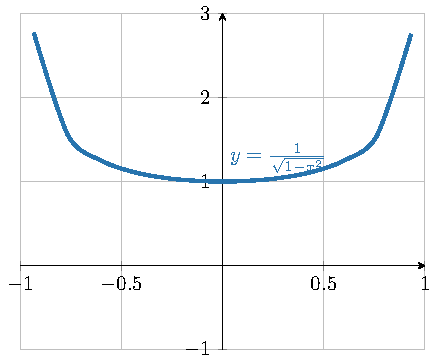
\includegraphics{chapters/4-IntegrationRn/figures/figures-undefinedonr.pdf}
        \end{center}
        Recall that $\int_{-1}^1 \frac{1}{\sqrt{1-x^2}} \ dx = \left[\arcsin{x}\right] \bigg|_{-1}^1 = \pi$.
    \end{example}

Thinking of the integral as the signed volume under the graph, we should expect $$\int_\R \frac{1}{\sqrt{1-x^2}} \ dx = \int_{-1}^1 \frac{1}{\sqrt{1-x^2}} \ dx = \pi$$

    We can make this precise using indicator functions!  

    \begin{definition}
     Let $A \subset \R^n$, and let $f : A \to \R$ be a function. We can extend $f$ to a function $\Tilde{f}(\bm{x}) : \R^n \to \R$ by defining
    $$\Tilde{f}(\bm{x}) := \left\{
		\begin{array}{ll}
			f(\bm{x}) & \text{ if } \bm{x} \in A \\
			0 & \text{ if } \bm{x} \notin A
		\end{array}
		\right.$$
        
    We will often use the following abusive notation when we want to indicate the domain $A$:
    $$f(\bm{x})1_A(\bm{x}) := \Tilde{f}(\bm{x})$$   
    \end{definition}

    

    \begin{definition}
    A function $f: A \subset \R^n \to \R$ is \textbf{integrable} if the function $f(\bm{x})1_A(\bm{x})$ is integrable, and we can define the integral of $f$ (denoted $\int_A f(\bm{x}) \ dV$) as

    $$\int_A f(\bm{x}) \ dV := \int_{\R^n} f(\bm{x})1_A(\bm{x}) \ dV$$
    
    \end{definition}

\begin{example}
    Let $f: (-1,1) \to \R$ be the function defined by $f(x) = \frac{1}{\sqrt{1-x^2}}$.  We can extend it to the function $\Tilde{f}(x) : \R \to \R$ by defining
    $$\Tilde{f}(x) := \left\{
		\begin{array}{ll}
			\frac{1}{\sqrt{1-x^2}} & \text{ if } \bm{x} \in (-1,1) \\
			0 & \text{else}
		\end{array}
		\right.$$
       
    \end{example}

    We can combine these two notions as well to define integrals of integrable functions $f : A \subset \R^n \to \R$ over regions $B \subset \R^n$.

    \begin{definition}
        Let $B \subset \R^n$, and let $f : A \subset \R^n \to \R$ be an integrable function. Then we can define the integral $\int_B f(\bm{x}) \ dV$ as

        $$\int_B f(\bm{x}) \ dV := \int_{\R^n} f(\bm{x})1_A(\bm{x})1_B(\bm{x}) \ dV$$
        
        By construction,

        \begin{align*}
        \int_B f(\bm{x}) \ dV &= \int_B \Tilde{f}(\bm{x}) \ dV \\
        &= \int_{\R^n} \Tilde{f}(\bm{x})1_B(\bm{x}) \ dV \\
        &= \int_{\R^n} f(\bm{x})1_A(\bm{x})1_B(\bm{x}) \ dV
    \end{align*}
    \end{definition}

\subsection{Properties of the integral}

In this section, we will prove some properties about the multivariable integral.  Recall that when you see integrability, you should think about continuous functions that are bounded with bounded support.

\begin{theorem}
    
    Let $f, g : \R^n \to \R$ be two integrable functions.  Then
    
    \begin{enumerate}
        \item $f+g$ is also integrable, and
        $$\int_{\R^n} f+g \ dV = \int_{\R^n} f \ dV + \int_{\R^n} g \ dV$$
        \item If $\lambda \in \R$, then $\lambda f$ is integrable, and 
        $$\int_{\R^n} \lambda f \ dV = \lambda \int_{\R^n} f \ dV$$
        \item If $f(\bm{x}) \leq g(\bm{x})$ for all $\bm{x} \in \R^n$, then $$\int_{\R^n} f \ dV \leq \int_{\R^n} g \ dV$$
        \item $|f|(\bm{x}) := |f(\bm{x})|$ is integrable, and $$\left|\int_{\R^n} f \ dV\right| \leq \int_{\R^n} |f| \ dV$$
    \end{enumerate}
    
    \end{theorem}

    \begin{corollary}
    We can reduce to studying integrals of non-negative functions.
    \end{corollary}
    
    \begin{definition}
    Given a function $f : \R^n \to \R$, we define two auxillary \textbf{non-negative functions}, $f^+$ and $f^-$.
    $$f^+(\bm{x}) := \left\{
		\begin{array}{ll}
			f(\bm{x}) & \text{ if } f(\bm{x}) \geq 0 \\
			0 & \text{ otherwise}
		\end{array}
		\right. \qquad f^-(\bm{x}) := \left\{
		\begin{array}{ll}
			-f(\bm{x}) & \text{ if } f(\bm{x}) \leq 0 \\
			0 & \text{ otherwise}
		\end{array}
		\right.$$
    
    \end{definition}

    \begin{example}
        Let $f(x) = x$. Then $$f^+(x) := \left\{
		\begin{array}{ll}
			x & \text{ if } x \geq 0 \\
			0 & \text{ otherwise}
		\end{array}
		\right. \qquad f^-(x) := \left\{
		\begin{array}{ll}
			-x & \text{ if } x \leq 0 \\
			0 & \text{ otherwise}
		\end{array}
		\right.
  $$

\begin{center}
      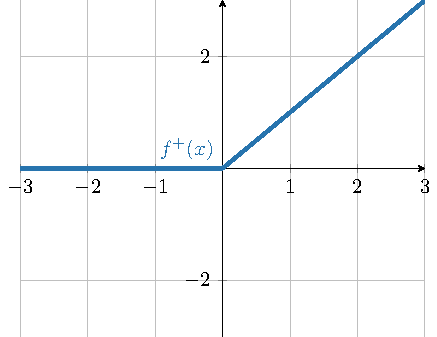
\includegraphics[scale=.8]{chapters/4-IntegrationRn/figures/figures-fplus.pdf}
      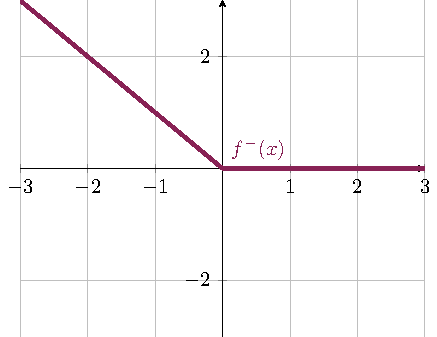
\includegraphics[scale=.8]{chapters/4-IntegrationRn/figures/figures-fminus.pdf}
\end{center}
    \end{example}
    
    \begin{proposition}
    $f(\bm{x}) = f^+(\bm{x}) - f^-(\bm{x})$.
    \end{proposition}


    \begin{proposition}
    Suppose that $f(\bm{x})$ is integrable on $\R^n$, and $g(\bm{y})$ is integrable on $\R^m$.  Then $h(\bm{x},\bm{y}) = f(\bm{x})g(\bm{y})$ is integrable on $\R^{n+m}$, and 
    $$\int_{\R^{n+m}} h \ dV \ dW = \int_{\R^n} f \ dV \int_{\R^n} g \ dW$$
    \end{proposition}
    
    \begin{remark}
        \textbf{Warning:} Note that $\bm{x}$ and $\bm{y}$ are necessarily different variables.  Furthermore, $$\int_{\R^{n}} f(\bm{x})g(\bm{x}) \ dV \neq \int_{\R^n} f(\bm{x}) \ dV \int_{\R^n} g(\bm{x}) \ dV$$
    \end{remark}

    \begin{example}
        Consider the functions $f(x) = x^2$, $g(x) = x$, and the region $A = [0,1] \subset \R$.  Observe that $$\int_0^1 f(x)g(x) \ dx = \int_0^1 x^3 \ dx \neq \left(\int_0^1 x^2 \ dx\right)\left(\int_0^1 x \ dx\right)$$
        The correct interpretation of the right hand side should be 
        $$\int_{A \times A} x^2y \ dA$$
        We will see how to calculate this in the next section.
    \end{example}
    
\subsection{Exercises}

\begin{problem}{examplesboundedboundedsupport}
Come up with examples of
       \begin{enumerate}
           \item a multivariable function that is not bounded
           \item a multivariable function that does not have bounded support
           \item A multivariable function that is neither bounded nor has bounded support.
       \end{enumerate}
\end{problem}

\begin{problem}{boundedboundedsupportvspace}
    Prove that if $f$ and $g$ are functions that are bounded with bounded support, then $f+g$ and $\lambda f$ are also functions that are bounded with bounded support.
\end{problem}

\begin{problem}{cube1}
    Explicitly describe and sketch the dyadic cube $C_{\langle1,1\rangle,2}$ in $\R^2$.
\end{problem}

\begin{problem}{cube2}
    Explicitly describe and sketch the dyadic cube $C_{\langle1,1,1\rangle,1}$ in $\R^3$.
\end{problem}

\begin{problem}
    Consider the subset $C_{\langle1,1\rangle,2}$ in $\R^2$, and let $f(x,y) = x^2 + y^2$.  Calculate $M_{C_{\langle1,1\rangle,2}}(f)$ and $m_{C_{\langle1,1\rangle,2}}(f)$.
\end{problem}


\begin{problem}{boundsdarboux}
    Prove that $U_N(f) \geq L_N(f)$.
\end{problem}

\begin{problem}{upperdarbouxexist}
    Let $f: \R^n \to \R$ be a continuous function that is bounded with bounded support. Prove that $U(f) := \lim_{N \to \infty} U_N(f)$ exists.  (You will need to use exercise \ref{problem:boundedincreasing}).
    
    \fixthis{reference problem}
\end{problem}

\begin{problem}{lowerdarbouxexist}
    Let $f: \R^n \to \R$ be a continuous function that is bounded with bounded support. Prove that $L(f) := \lim_{N \to \infty} L_N(f)$ exists. (You will need to use exercise \ref{problem:boundeddecreasing}).
\end{problem}

\begin{problem}{riemannintegrabletodarboux}
    Let $\bm{R_{k,N}} \in C_{\bm{k},N}$ be an arbitrary sampling of the dyadic partition, and define 
    $$R_N(f) := \sum_{C \in D_N(\R^n)} f(\bm{R_{k,N}}) \textnormal{vol(C)}$$
    
    Prove that if $f$ is integrable, then
    $$\lim_{N\to\infty} R_N(f) = \int_{\R^n}f \ dV $$

    (\textbf{Hint:} use the squeeze theorem!)
\end{problem}


\begin{problem}{strictineq}
    Give an example of an integrable function $f$ such that $$\left|\int_{\R^n} f \ dV\right| < \int_{\R^n} |f| \ dV$$
    (that is, an example of strict inequality)
\end{problem}

\begin{problem}{supfg}
    Let $f,g : \R^n \to \R$ be integrable functions, and consder the function $\sup(f,g)$ defined by $$\sup(f,g)(\bm{x}) := \sup(f(\bm{x},g(\bm{x})$$ Show that $\sup(f,g)$ is integrable.
    (\textbf{Hint:} Write $\sup(f,g)$ in terms of $f^+,f^-,g^+,g^-$).
\end{problem}

\begin{problem}{inffg}
    Let $f,g : \R^n \to \R$ be integrable functions, and consder the function $\inf(f,g)$ defined by $$\inf(f,g)(\bm{x}) := \inf(f(\bm{x},g(\bm{x})$$ Show that $\inf(f,g)$ is integrable.
    (\textbf{Hint:} Write $\inf(f,g)$ in terms of $f^+,f^-,g^+,g^-$).
\end{problem}



\section{Calculating multivariable integrals}

    \begin{motivating}
        Given a region $B \subset \R^n$ and an integrable function $f$, how can we compute $\int_B f(\bm{x}) \ dV$?
    \end{motivating}

    \begin{theorem}[Fubini]
    Let $f(\bm{x}): \R^n \to \R$ be a continuous function that is bounded with bounded support, and let $(i_1, \cdots i_n)$ be a permutation of the set $\{1, \cdots, n\}$. Then 
    
    $$\int_{\R^n} f(\bm{x}) \ dV = \int_{-\infty}^{\infty} \left( \cdots \left(\int_{-\infty}^{\infty} f(\bm{x}) \ dx_{i_1} \right) \cdots \right) \ dx_{i_n}$$

    \end{theorem}

    That is, we can compute an integral $\int_{\R^n} f(\bm{x}) \ dV$ as an iterated integral, in any variable order!

    \begin{example}
        Let $R$ be the region $[0,1] \times [0,1]$.  Compute the integral 
        $$\iint_R xe^{xy} \ dA $$
        By Fubini's theorem, there are two iterated integrals we can use (namely, $\int_0^1\int_0^1 xe^{xy} \ dx \ dy$ or $\int_0^1\int_0^1 xe^{xy} \ dy \ dx$).  

        However, observe that the former requires integration by parts.  However, we can compute 
        \begin{align*}
            \iint_R xe^{xy} \ dA  &= \int_0^1\int_0^1 xe^{xy} \ dy \ dx \\
            &= \int_0^1 [e^{xy}] \bigg|_{y=0}^{y=1} \ dx \\
            &= \int_0^1 e^{x}-1 \ dx \\
            &= e-2
        \end{align*}
        
    \end{example}


    \begin{remark}
        \fixthis{Relationship to Clairaut's theorem} (see corollary \ref{clairautcorollary}).
    \end{remark}

    Typically, the most difficult thing to do in multivariable integration is to visualize the region that you're integrating over.  

    \begin{example}
        Compute the volume of the solid region enclosed between the graph of  $f(x,y) = y$ and the $xy$-plane, over the region below:

        \begin{example}
            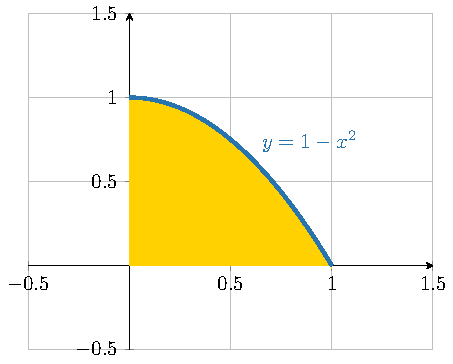
\includegraphics[scale=.7]{chapters/4-IntegrationRn/figures/figures-1-xsquaredregion.pdf}
        \end{example}
        
    \end{example}

    \begin{example}
    Calculate the integral of $f(x,y,z) = xyz$ over the region $W$ in the first octant (that is, $x, y, z \geq 0$) bounded by $z = 4 - y^2$, $z = 0$, $y = 2x$, and $x= 0$.

    We can sketch this region as the region between $z=0$ and the parabolic cylinder ($z = 4 - y^2$), sitting above the triangle cut out by $x=0$, $y = 2x$, and $y=2$. We can thus write the region $W$ as 
    $$\{(x,y,z) \ | \ 0 \leq z \leq 4-y^2, 0 \leq x \leq \frac{y}{2}, 0 \leq y \leq 2\}$$
    Thus, we can compute the integral as $$\int_0^2\int_0^\frac{y}{2}\int_0^{4-y^2} xyz \ dz \ dx \ dy = \frac{2}{3}$$

    Alternatively, we can sketch this region as the region between $x=0$ and the plane $x = \frac{y}{2}$, sitting above the parabola cut out by $z = 4 - y^2$, $z=0$, and $y=0$.  We can thus write the region $W$ as 
    $$\{(x,y,z) \ | \ 0 \leq x \leq \frac{y}{2}, 0 \leq z \leq 4-y^2, 0 \leq y \leq 2\}$$
    Thus, we can also compute the integral as $$\int_0^2\int_0^{4-y^2}\int_0^\frac{y}{2} xyz \ dx \ dz \ dy = \frac{2}{3}$$

    As Clairaut's theorem stipulates, we can choose the iterated integral in the order that we want.
    \end{example}

    \begin{example}
        Compute the integral of $f(x,y) = \frac{1}{\ln(x)}$ over the domain $D$ bounded by $x = e^y$ and $x= e^{\sqrt{y}}$.

    \begin{center}
        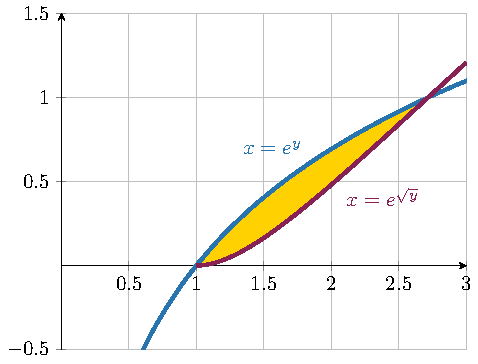
\includegraphics{chapters/4-IntegrationRn/figures/figures-intersectfubini.pdf}
    \end{center}
        
    \end{example}

\begin{theorem}[Decomposition of Domains]
        Let $K$ be a compact (closed and bounded) subset in $\R^n$ such that its boundary $\partial D$ has volume zero.  Furthermore, let $K = K_1 \cup K_2$, such that $K_1$ and $K_2$ are compact, and the intersection $K_1 \cap K_2$ has volume 0\footnote{Typically, $K_1 \cap K_2$ will be an ($n-1$)-dimensional subset (like the graph of a function $f : \R^{n-1} \to \R$, as in theorem \ref{thm:graphvolume0})}. 
    
    
    Let $f : K \to \R$ be a continuous function.  Then $f$ is integrable over $K_1$ and $K_2$, and 
    $$\int_K f(\bm{x}) \ dA = \int_{K_1} f(\bm{x}) \ dA + \int_{K_2} f(\bm{x}) \ dA $$ 
    \end{theorem}

\begin{example}
    Evaluate the double integral of $f(x,y) = 1-2x$ over the region $K$ as drawn below:

    \begin{center}
        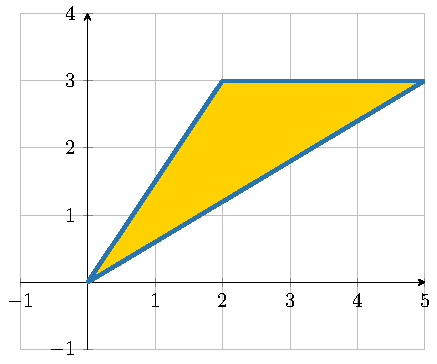
\includegraphics{chapters/4-IntegrationRn/figures/figures-decomposek.pdf}
    \end{center}

    We can decompose $K$ into two regions, $K_1$ and $K_2$ defined as $$K_1 = \{(x,y) \ | \ 0 \leq x \leq 2, \frac{3}{5}x \leq y \leq \frac{3}{2}x\}$$ and 
    $$K_2 = \{(x,y) \ | \ 2 \leq x \leq 5, \frac{3}{5}x \leq y \leq 3 \}$$  
    Note that $K_1$ and $K_2$ are both \textbf{vertically simple} (which simplifies calculating the integral). 

    \begin{center}
        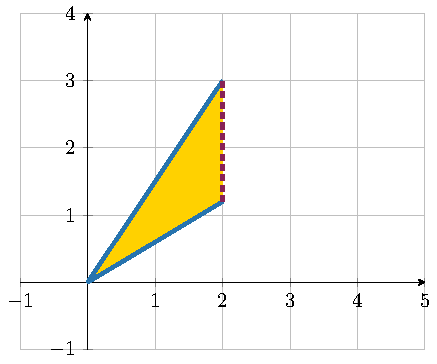
\includegraphics{chapters/4-IntegrationRn/figures/figures-decomposek1.pdf}
        The region $K_1$
        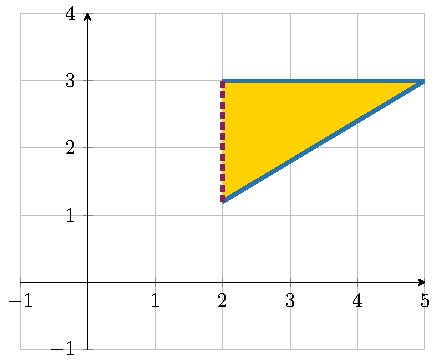
\includegraphics{chapters/4-IntegrationRn/figures/figures-decomposek2.pdf}
        The region $K_2$
    \end{center}

    Observe that $K = K_1 \cup K_2$, and the intersection $K_1 \cap K_2$ is the curve $\{(x,y) \ | \ \frac{6}{5} \leq y \leq 3, x=2 \}$, which has volume 0.
    Therefore, 
    \begin{align*}
        \iint_K 1-2x \ dA &= \iint_{K_1} 1-2x \ dA + \iint_{K_2} 1-2x \ dA\\
        &= \int_0^2\int_{\frac{3}{5}x}^{\frac{3}{2}x} 1-2x \ dy \ dx + \int_2^5\int_{\frac{3}{5}x}^{3} 1-2x \ dy \ dx \\
        &= \int_0^2 (1-2x)(\frac{3}{2}x-\frac{3}{5}x) \ dx + \int_2^5 (1-2x)(3-\frac{3}{5}x) \ dx \\
        &= -3 + -13.5 = -16.5        
    \end{align*}
    
    
    
\end{example}

\begin{definition}
    A subset $D \subset \R^2$ is \textbf{vertically simple}\define{vertically simple} if it is the region between graphs of two continuous functions $y = g_1(x)$ and $y = g_2(x)$ over a fixed interval of $x$-values $[a,b]$.
\end{definition}

\begin{example}
   The regions $K_1 = \{(x,y) \ | \ 0 \leq x \leq 2, \frac{3}{5}x \leq y \leq \frac{3}{2}x\}$ and $K_2 = \{(x,y) \ | \ 2 \leq x \leq 5, \frac{3}{5}x \leq y \leq 3 \}$ are both \textbf{vertically simple}. 
\end{example}

\begin{definition}
    A subset $D \subset \R^2$ is \textbf{horizontally simple}\define{horizontally simple} if it is the region between graphs of two continuous functions $x = h_1(y)$ and $x = h_2(y)$  over a fixed interval of $y$-values $[c,d]$.
\end{definition}

\begin{example}
    The region $K = \{(x,y) \ | \ \frac{2}{3}y \leq x \leq \frac{5}{3}y, 0 \leq y \leq 3\}$ is horizontally simple.  \textbf{Warning:} Be careful about the inequalities!

    We could therefore have instead computed 
    \begin{align*}
        \iint_K 1-2x \ dA &= \int_0^3\int_{\frac{2}{3}y}^{\frac{5}{3}y} 1-2x \ dx \ dy \\
        &= \int_0^3 [x-x^2] \bigg|_{\frac{2}{3}y}^{\frac{5}{3}y} \ dy\\
        &= \int_0^3 \frac{5}{3}y - (\frac{5}{3}y)^2 - \frac{2}{3}y + (\frac{2}{3}y)^2 \ dx \\
        &= -16.5        
    \end{align*}
\end{example}

\subsection{Exercises}

\begin{problem}{int1}
    Let $R$ be the region $[1,2] \times [2,4]$.  Compute the integral 
        $$\iint_R e^{3x-y} \ dA = \int_1^2\int_2^4 e^{3x-y} \ dy \ dx$$
\end{problem}

\begin{problem}{fub1}
    Let $R$ be the region $[0,1] \times [0,1]$.  Compute the integral 
        $$\iint_R xe^{xy} \ dA $$
\end{problem}

\begin{problem}{int3}
    Compute the integral $\iint_R x^2\tan(y) \ dA$ for $R$ the rectangle $[0,2] \times [0, \frac{\pi}{3}]$
\end{problem}

\begin{problem}{int4}
    Compute the integral $\iint_R \frac{x}{1+xy} \ dA$ for $R$ the rectangle $[0,1] \times [0, 1]$
\end{problem}

\begin{problem}{int5}
    Find the volume of the solid region enclosed between the graph of  $f(x,y) = \frac{1}{\sqrt{x+y}}$ and the $xy$-plane, over the rectangle $[0,4] \times [0,5]$.	
\end{problem}

\begin{problem}{fub2}
    Compute the integral of $f(x,y) = \frac{1}{\ln(x)}$ over the domain $D$ bounded by $x = e^{4y}$ and $x= e^{2\sqrt{y}}$.
\end{problem}

\begin{problem}{int6}
    Find the volume of the region bounded by $y = 1-x^2$, $z = 1$, $y = 0$, and $z+y=2$.
\end{problem}

\begin{problem}{symmetry}
    The volume of a sphere of radius 2 is $\frac{32\pi}{3}$.  What is the value of the following integral?$$\int_{-\frac{\pi}{4}}^{\frac{\pi}{4}}\int_0^\pi\int_0^2 \rho^2 \sin(\phi) \ d\rho \ d\phi \ d\theta$$
\end{problem}

\begin{problem}{3dint1}
    Integrate $f(x,y,z) = x$ over the region $W$ bounded above by $z = 4-x^2-y^2$ and below by $z=x^2+3y^2$ in the octant $x \geq 0$, $y \geq 0$, $z \geq 0$.
\end{problem}

\begin{problem}{3dint2}
    Find the volume between the intersection of the surfaces $z = x^2 + y^2$ and $z = 10 - x^2 - y^2$.
\end{problem}

\begin{problem}{3dint3}
    Compute $\iiint_W x \ dV$, where $W$ is the region in the first octant below the planes $z = 1-x$ and $z = 3 - x- y$.
\end{problem}










\section{Integrability}\label{sec:integrability}

In the previous sections, we have defined the notion of integrability, which we will restate below:

\begin{definition}
    Let $f: \R^n \to \R$ be a bounded function with bounded support.
    We say that $f$ is \textbf{integrable} if $U(f) = L(f)$.
    
    The \textbf{integral} of $f$ is $$\int_{\R^n} f(\bm{x}) \ dV := U(f) = L(f)$$

    Equivalently \fixthis{ref}, for any $\varepsilon > 0$,
    there exists $N$ such that $|U_N(f) - L_N(f)| < \varepsilon$
    \end{definition}

The examples we've had so far are the following:
        
    \begin{theorem}
     If $f : \R^n \to \R$ is a continuous function that is bounded with bounded support, then $f$ is integrable.   
    \end{theorem}


    \begin{definition}
    Let $f: \R^n \to \R$ be a function, and let $A \subset \R^n$.  The \textbf{oscillation} of $f$ over $A$ is defined as $$\text{osc}_A(f) := M_A(f) - m_A(f)$$
    \end{definition}

    \begin{center}
        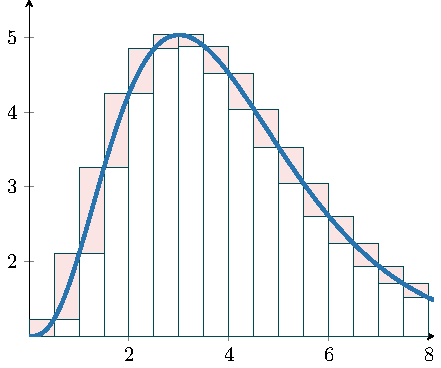
\includegraphics{chapters/4-IntegrationRn/figures/figures-integraloscillation.pdf}
    \end{center}
    
    \begin{theorem}
    A function $f: \R^n \to \R$ is integrable if and only if
    \begin{enumerate}
        \item $f$ is bounded with bounded support
        \item For all $\varepsilon > 0$, there exists $N$ such that $$\sum_{\{C \in D_N \ | \ \text{osc}_C(f) > \varepsilon \}} \textnormal{vol}_n C < \varepsilon$$
    \end{enumerate}
    \end{theorem}

\begin{proof}
    fixthis
\end{proof}

\begin{example}
    The indicator function on the unit disk
\end{example}

\begin{example}

The function $\sin(\frac{1}{x})$
    
%     \begin{center}
    
%     \begin{tikzpicture}[x=8cm]
%     \draw[xstep=.2,ystep=.5,lightgray,ultra thin] (-0.1,-1.5) grid (1.1,1.5);
%     \draw[->] (0,0) -- (1.1,0) node[right] {$x$};
%     \draw[->] (0,-1) -- (0,1.1) node[above] {$y$};
%   \draw[blue,domain=0.01:1,samples=5000] plot (\x, {sin((1/\x)r)});
% \end{tikzpicture}    
%     \end{center}
    
\end{example}

















\subsection{Exercises}

\begin{problem}{integrabilitycounterexamples1}
Come up with (and prove) an example of a function that is not integrable.
\end{problem}

\begin{problem}{integrabilitycounterexamples2}
Come up with (and prove) an example of a function where $|f|$ is integrable, but $f$ is not integrable.
\end{problem}

\section{Change of variables}

\subsection{Polar, cylindrcial, and spherical coordinate}

\subsection{General Change of Variables}

\fixthis{recall Jacobian}




\begin{theorem}[The change of variables formula in $\R^2$]
    Let  $G(u,v) = \left(x(u,v), y(u,v)\right)$ be a map such that
    
    \begin{enumerate}
        \item $G$ sends a region $D_0$ to $D$.  
        \item $G$ is a $C^1$ mapping.
        \item $G$ is one-to-one on the interior of $D_0$.  
    \end{enumerate}

    
    If $f(x,y)$ is continuous, then
    $$\iint_D f(x,y) \ dx \ dy = \iint_{D_0} f(x(u,v), y(u,v)) \left|\textnormal{Jac}(G)\right| \ du \ dv$$
    
\end{theorem}

\begin{example}
    Polar coordinates map defined by $$G(r,\theta) = (r\cos(\theta), r\sin(\theta))$$
\end{example}

\begin{remark}
    Sometimes, it is easier to find a map going in the \textit{wrong direction}, $$F(x,y) = (u(x,y),v(x,y))$$
    Then $G = F^{-1}$.
    \end{remark}
    
    %     \begin{center}
    %     \includegraphics[scale=0.45]{pictures/map.png}
    % \end{center}
    
    \begin{theorem}
    If $G = F^{-1}$, and $\textnormal{Jac}(F) \neq 0$, then $\textnormal{Jac}(G) = \frac{1}{\textnormal{Jac}(F)}$
    \end{theorem}










    \begin{theorem}[Change of variables]
    Let $K \subset \R^n$ be a compact set such that $\text{vol}_n(\partial K) = 0$.  Let $U \subset \R^n$ be an open set containing $K$. Let $$\Phi : U \to \R^n$$ be a map such that 
    \begin{enumerate}
        \item $\Phi$ is a $C^1$ mapping.
        \item $\Phi$ is injective on the interior of $K$.  
        \item $\det [D(\Phi)] \neq 0$ on the interior of $K$.  
    \end{enumerate}
    Then if $f: \Phi(K) \to \R$ is a continuous function, then 
    $$\int_{\Phi(K)} f \  dV = \int_K(f \circ \Phi) \cdot |\det [D(\Phi)]| \ dV$$
    \end{theorem}

    \fixthis{examples that show necessity}

    \subsection{Exercises}

    \begin{problem}{polar1}
    Compute the integral $$\int_0^3\int_0^{\sqrt{9-y^2}}\int_0^1 z\sqrt{x^2 + y^2} \ dz \ dx \ dy$$
\end{problem}

\begin{problem}{change1}
    Let $D$ be the region in the first quadrant defined by $$D = \{ (x,y) \ | \ 1 \leq xy \leq 4, 1 \leq y/x \leq 4 \}$$
    Compute $\iint_D (x^2 + y^2) \ dx \ dy$.
\end{problem}

\begin{problem}{change2}
    \begin{subproblems}
    \item Consider the parallelogram $P$ with vertices $A = (0,0)$, $B = (3,1)$, $C = (2,3)$, $D = (5,4)$.  Find a change of variables $G(u,v) = (x(u,v), y(u,v))$ that transforms the unit square to $P$.  Compute the determinant of the Jacobian of $G$.
    \item Use your work from the previous problem to compute the integral $$\iint_P e^{3x-y} \ dA$$.
    \end{subproblems}
    
\end{problem}

\begin{problem}{change3}
    Consider the change of variables $G(u,v) = (uv^{-1}, uv)$ that transforms the square $[1,2]\times[1,2]$ to the region $D$ in the first quadrant bounded by $1 \leq xy \leq 4$ and $1 \leq \frac{y}{x} \leq 4$. Use this to compute the integral $$\iint_D x^2+y^2 \ dA$$.
\end{problem}